%        File: arfc-pres.tex
%     Created: 2018-12-15 10:00 AM 2018 C
%


%\documentclass[11pt,handout]{beamer}
\documentclass[9pt,handout]{beamer}
\hypersetup{colorlinks,allcolors=.,urlcolor=orange}
\usetheme[white]{Illinois}
%\title[short title]{long title}
\title[Multiphysics in MSRs]{Multiphysics in MSRs}
%\subtitle[short subtitle]{long subtitle}
%\author[short name]{long name}
\author[Huff]{Kathryn Huff\\Advanced Reactors and Fuel Cycles Group\\University 
of Illinois at Urbana-Champaign}
%\date[short date]{long date}
\date[05.13.2021]{May 13, 2021}
%\institution[short name]{long name}
\institute[UIUC]{University of Illinois at Urbana-Champaign}
\institute[OSU]{Oregon State University Colloquium}

\usepackage{lmodern}
%\usepackage{bbding}
\usepackage{amsfonts}
\usepackage{amsmath}
\usepackage{xspace}
\usepackage{graphicx}
%\usepackage{caption}  % allows center figures caption
\usepackage{notoccite}
\usepackage{animate}
\usepackage{subfigure}
\usepackage{booktabs} % nice rules for tables
\usepackage{microtype} % if using PDF
\usepackage{bigints}
\newcommand{\units}[1] {\:\text{#1}}%
\newcommand{\SN}{S$_N$}%{S$_\text{N}$}%{$S_N$}%
\DeclareMathOperator{\erf}{erf}
%I need some complimentary error funcitons... 
\DeclareMathOperator{\erfc}{erfc}
%Those icons in the references are terrible looking
\setbeamertemplate{bibliography item}[text]

%%%% Acronym support

\usepackage[acronym,toc]{glossaries}
\include{acros}

\makeglossaries

%try to get rid of header on title page\dots
\makeatletter
    \newenvironment{withoutheadline}{
        \setbeamertemplate{headline}[default]
        \def\beamer@entrycode{\vspace*{-\headheight}}
    }{}
\makeatother

\makeatother
\setbeamertemplate{footline}
{
  \leavevmode%
  \hbox{%
    \rightline{\insertframenumber{} / \inserttotalframenumber\hspace*{1ex}}
  }%
  \vskip0pt%
}
\makeatletter
\begin{document}
%%%%%%%%%%%%%%%%%%%%%%%%%%%%%%%%%%%%%%%%%%%%%%%%%%%%%%%%%%%%%
%% From uw-beamer Here's a handy bit of code to place at 
%% the beginning of your presentation (after \begin{document}):
\newcommand*{\alphabet}{ABCDEFGHIJKLMNOPQRSTUVWXYZabcdefghijklmnopqrstuvwxyz}
\newlength{\highlightheight}
\newlength{\highlightdepth}
\newlength{\highlightmargin}
\setlength{\highlightmargin}{2pt}
\settoheight{\highlightheight}{\alphabet}
\settodepth{\highlightdepth}{\alphabet}
\addtolength{\highlightheight}{\highlightmargin}
\addtolength{\highlightdepth}{\highlightmargin}
\addtolength{\highlightheight}{\highlightdepth}
\newcommand*{\Highlight}{\rlap{\textcolor{HighlightBackground}{\rule[-\highlightdepth]{\linewidth}{\highlightheight}}}}
%%%%%%%%%%%%%%%%%%%%%%%%%%%%%%%%%%%%%%%%%%%%%%%%%%%%%%%%%%%%%
%%--------------------------------%%
\begin{withoutheadline}
\frame{
  \titlepage
}
\end{withoutheadline}

%%--------------------------------%%
\AtBeginSection[]{
\begin{frame}
  \frametitle{Outline}
  \tableofcontents[currentsection]
\end{frame}
}

\section{Intro}

\begin{frame}
  \frametitle{Insights at Disparate Scales}
               \begin{figure}[t]
                \vspace*{-0.1in}
			\hspace*{-0.35in}
                \includegraphics[height=0.5\textwidth]{./images/synergy.png}
               \end{figure}            
\end{frame}

\begin{frame}
  \frametitle{Challenges in Liquid-Fueled Reactor Simulation}
                  \vspace*{-0.05in}
               \begin{enumerate}
                \item Contemporary burnup codes cannot treat fuel movement.
                \item Neutron precursor locations drift before neutron emission.
                \item Operational and safety parameters change during reactor operation.
                \item Neutronics and thermal hydraulics are tightly interdependent.
               \end{enumerate}

           \begin{figure}[t]
                \vspace*{-0.05in}
			\hspace*{-0.2in}
                \includegraphics[height=0.47\textwidth]{./images/coupled_physics.png}
		\vspace*{-0.05in}
		\caption{Challenges in simulating \glspl{MSR} (Image courtesy of Manuele Aufiero, 2012).}
     	 \end{figure}               
\end{frame}

%\begin{frame}
%  \frametitle{Approaches}
%                  \vspace*{-0.1in}
%              \begin{block}{Point Reactor Kinetics \cite{huff_pyrk:_2015}}
%                Only appropriate for stationary or nearly stationary fuels.
%              \end{block}
%
%              \begin{block}{Simulation of online reprocessing and depletion 
%                      (SaltProc)\cite{rykhlevskii_arfc/saltproc:_2018,rykhlevskii_online_2017}}
%               \begin{enumerate}
%                \item Create high-fidelity full-core neutronics model of the 
%                        core neutronics can be necessary for reducing 
%                               compounding error.
%                \item SaltProc wraps SERPENT monte carlo neutron transport for 
%                        simulation of liquid fuel reprocessing.
%                \item Enables day-to-day rsolution off neutronics and reprocessing modeling 
%                        over many decades of depletion and fuel cycle performance.
%               \end{enumerate}
%               \end{block}
%
%              \begin{block}{Multiphysics simulation of \gls{MSR} (Moltres)\cite{lindsay_introduction_2018}}
%               \begin{enumerate}
%                \item Steady-state and transient coupling of neutron fluxes, 
%                        precursor drift, and thermal-hydraulics.
%                \item Incorporates advective movement of delayed neutron precursors.
%                \item 2D axisymmetric and 3D geometries supported.
%               \end{enumerate}
%               \end{block}
%
%\end{frame}

\subsection{Molten Salt Reactors}
\begin{frame}
        \frametitle{Types of Molten Salt Reactors}
        \begin{block}{Stationary Fuel}
                \begin{itemize}
                        \item Prismatic graphite block with TRISO fuel and 
                                coolant channels (e.g. FHR DR, TMSR-SF1). Clean salt 
                                coolant.
                        \item Stationary TRISO pebble matrix (e.g. TMSR-SF)
                \end{itemize}

        \end{block}
        \begin{block}{Mobile Fuel}
                \begin{itemize}
                        \item Mobile solid fuel elements, such as pebbles. 
                                Clean salt coolant. (e.g. PB-FHR/Kairos)
                        \item Non-circulating fuel salt, ``can-type''. (e.g. Terrapower MCFR)
                        \item Circulating fuel salt ``pool-type''. (e.g. MSRE, MSBR, MSFR, 
                                Terrestrial MSR, TAP MSR, etc.)
                \end{itemize}
        \end{block}
\end{frame}

\begin{frame}
        \frametitle{Stationary Solid Fuel}
               \begin{figure}[t]
                \vspace*{-0.1in}
                \includegraphics[height=0.5\textwidth]{./images/example-ahtr.png}
                       \caption{The \gls{AHTR} \cite{forsberg_fuel_2004} 
                       is an example of a fluoride salt cooled reactor 
                       design fueled by a \textbf{stationary}, \textbf{solid} 
                       prismatic graphite TRISO compacts, and cooled by clean fluoride salt.
                       Image source \cite{gentry_burnable_2015}. }
               \end{figure}            
\end{frame}

\begin{frame}
        \frametitle{Mobile Solid Fuel}
               \begin{figure}[t]
                \vspace*{-0.1in}
                \includegraphics[height=0.2\textwidth]{./images/example-pbfhr-fuel.png}
                \includegraphics[height=0.4\textwidth]{./images/example-pbfhr-core.jpg}
                       \caption{The \gls{PBFHR} is an example reactor design 
                       fueled by \textbf{solid}, \textbf{mobile} graphite 
                       pebbles, with TRISO particles embedded in them. Image 
                       source \cite{andreades_technical_2014}.}
               \end{figure}            
\end{frame}

\begin{frame}
        \frametitle{Mobile, Non-Circulating, Liquid Fuel}
               \begin{figure}[t]
                \vspace*{-0.1in}
                \includegraphics[height=0.5\textwidth]{./images/example-mcfr.jpg}
                       \caption{The \gls{MCFR} from TerraPower is an example 
                       reactor design with \textbf{liquid}, \textbf{mobile}, 
                       \textbf{non-circulating} chloride salt fuel. Image 
                       source \cite{terrapower_llc_mcfr_2018,doene_southern_2018}.}
               \end{figure}            
\end{frame}


\begin{frame}
        \frametitle{Mobile, Circulating, Liquid Fuel}
               \begin{figure}[t]
                \vspace*{-0.1in}
                \includegraphics[height=0.5\textwidth]{./images/example-msbr.png}
                       \caption{The \gls{MSBR} \cite{robertson_conceptual_1971} is an example 
                       reactor design with \textbf{liquid}, \textbf{mobile}, 
                       \textbf{circulating} fluoride salt fuel, including 
                       breeding behavior due to varying channel shapes and 
                       sizes. Image 
                       source \cite{rosenthal_molten-salt_1970}.}
               \end{figure}            
\end{frame}

\begin{frame}
  \frametitle{Why Molten Salt Reactors?}
                  \vspace*{-0.1in}
              \begin{block}{Main advantages of liquid-fueled \glspl{MSR} \cite{elsheikh_safety_2013}}
               \begin{enumerate}
                \item High coolant temperature (600-750$^{\circ}$C).
                \item Various fuels can be used ($^{235}$U, $^{233}$U, Thorium, U/Pu).
                \item Increased inherent safety.
                \item High fuel utilization $\Rightarrow$ less nuclear waste generated.
                \item Online reprocessing and refueling.
               \end{enumerate}
               \end{block}
                  \vspace*{-0.1in}               
               \begin{block}{Main advantages of \gls{MSBR} \cite{robertson_conceptual_1971}}
               \begin{enumerate}
                \item Produces more fissile material than it consumes (breeding ratio 1.06).
                \item Thorium cycle limits plutonium and minor actinides.
                \item Could transmute spent fuel from existing \gls{NPP}.
               \end{enumerate}
               \end{block}

\end{frame}

\begin{frame}
  \frametitle{Challenges in Liquid-Fueled Reactor Simulation}
                  \vspace*{-0.05in}
               \begin{enumerate}
                \item Contemporary burnup codes cannot treat fuel movement.
                \item Neutron precursor locations drift before neutron emission.
                \item Operational and safety parameters change during reactor operation.
                \item Neutronics and thermal hydraulics are tightly interdependent.
               \end{enumerate}

           \begin{figure}[t]
                \vspace*{-0.05in}
			\hspace*{-0.2in}
                \includegraphics[height=0.47\textwidth]{./images/coupled_physics.png}
		\vspace*{-0.05in}
		\caption{Challenges in simulating \glspl{MSR} (Image courtesy of Manuele Aufiero, 2012).}
     	 \end{figure}               
\end{frame}

\begin{frame}
  \frametitle{Approaches}
                  \vspace*{-0.1in}
              \begin{block}{Point Reactor Kinetics}
                      PyRK \cite{huff_pyrk:_2015}, for example, is only appropriate for stationary or nearly stationary fuels.
              \end{block}

              \begin{block}{Multiphysics simulation of \gls{MSR} (Moltres)\cite{lindsay_introduction_2018}}
               \begin{enumerate}
                \item Steady-state and transient coupling of neutron fluxes, 
                        precursor drift, and thermal-hydraulics.
                \item Incorporates advective movement of delayed neutron precursors.
                \item 2D axisymmetric and 3D geometries supported.
               \end{enumerate}
               \end{block}

              \begin{block}{Simulation of online reprocessing and depletion 
                      (SaltProc)\cite{rykhlevskii_arfc/saltproc:_2018,rykhlevskii_online_2017}}
               \begin{enumerate}
                \item Create high-fidelity full-core neutronics model of the 
                        core neutronics can be necessary for reducing 
                               compounding error.
                \item SaltProc wraps SERPENT monte carlo neutron transport for 
                        simulation of liquid fuel reprocessing.
                \item Enables day-to-day rsolution off neutronics and reprocessing modeling 
                        over many decades of depletion and fuel cycle performance.
               \end{enumerate}
               \end{block}


\end{frame}


\subsection{Neutron Kinetics}
	
\begin{frame}
\frametitle{Fission}
  \begin{figure}[t]
   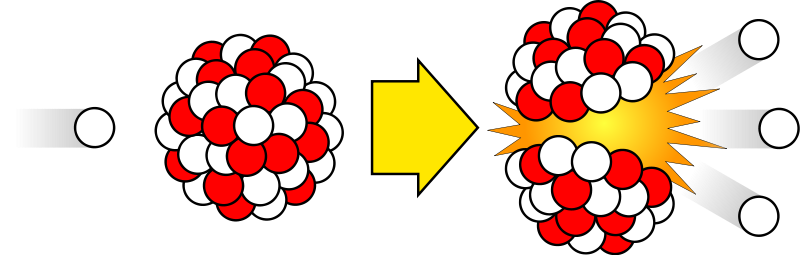
\includegraphics[width=\textwidth]{./images/fission.png}
	\caption{Cross sections: $\sigma(E,\vec{r},\hat{\Omega},T,x,i)$}
	\end{figure}
\end{frame}


\begin{frame}
\frametitle{Fission Chain Reaction}
  \begin{figure}[t]
   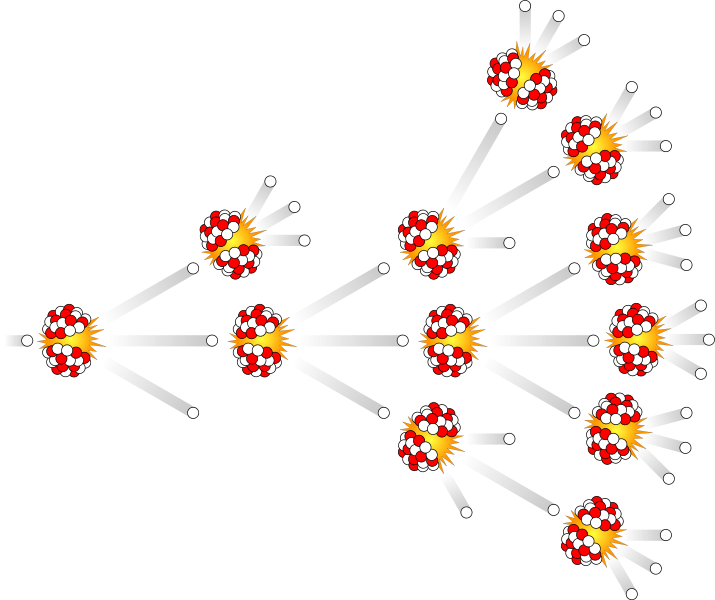
\includegraphics[height=0.75\textheight]{./images/fission-chain.png}
	\caption{Criticality: $k=1$}
	\end{figure}
\end{frame}

\begin{frame}
\frametitle{Reactivity}
		     \begin{align*}
		     k &= \mbox{"neutron multiplication factor"}\\
		     &= \frac{\mbox{neutrons causing fission}}{\mbox{neutrons produced by fission}}\\
		     \rho &= \frac{k-1}{k}\\
		     \rho &= \mbox{reactivity}\\
		     \end{align*}
\end{frame}

\begin{frame}
\frametitle{Feedback}
  \begin{figure}[t]
   \includegraphics[width=0.75\textwidth]{./images/feedback.png}
	\end{figure}
\end{frame}


\begin{frame}
\frametitle{Kinetics with Delayed Neutrons}
  \begin{figure}[t]
   \includegraphics[height=0.75\textheight]{./images/delayed_neutron.png}
	\caption{Delayed neutron fraction, $\beta_i$, and corresponding decay constant, $\lambda_{d,i}$.}
	\end{figure}
\end{frame}


\section{Point Kinetics \& TH Coupling}
\input{pyrk}
\section{MOOSE Framework}
\begin{frame}
  \frametitle{MOOSE Framework}
  \begin{columns}
    \column[t]{6cm}
  \begin{figure}[t]
     \vspace{-0.25in}
       \hspace*{-0.25in}
       \includegraphics[height=0.65\textheight]{./images/moose.png}
            \caption{Multi-physics Object-Oriented Simulation Environment 
            (MOOSE) 
            \cite{gaston_physics-based_2015,permann2020moose,lindsay2021automatic}.}
  \end{figure}
        \column[t]{4cm}
          \begin{itemize}
                  \item Developed by Idaho National Laboratory 
                          \cite{gaston_physics-based_2015,permann2020moose,lindsay2021automatic}
                  \item Framework is truly open source (LGPL)
                  \item Accessible docs and tutorials at \url{https://mooseframework.inl.gov}
                  \item Source code at \url{https://github.com/idaholab/moose}
          \end{itemize}

  \end{columns}
\end{frame}



\begin{frame}
        \frametitle{MOOSE Apps \& Kernels}
  \begin{columns}
    \column[t]{6cm}
  \begin{figure}[t]
     \vspace{-0.25in}
       \hspace*{-0.25in}
       \includegraphics[height=0.65\textheight]{./images/moose.png}
            \caption{Multi-physics Object-Oriented Simulation Environment (MOOSE).}
  \end{figure}
        \column[t]{4cm}
          \textbf{Lots of Open Kernels}
           \footnotesize{\begin{itemize} 
                \item Chemical reactions
                \item Contact
                \item Fluid Properties
                \item Functional Expansion Tools
                \item Geochemistry
                \item Heat Conduction
                \item Level Set
                \item Navier-Stokes
                \item Peridynamics
                \item Phase Field
                \item Porous Flow
                \item Ray Tracing
                \item Reconstructed Discontinous Galerkin
                \item Tensor Mechanics
                \item \ldots
          \end{itemize}
          }
  \end{columns}
\end{frame}

\begin{frame}
        \frametitle{MOOSE Apps \& Kernels}
  \begin{columns}
    \column[t]{6cm}
  \begin{figure}[t]
     \vspace{-0.25in}
       \hspace*{-0.25in}
       \includegraphics[height=0.65\textheight]{./images/moose.png}
            \caption{Multi-physics Object-Oriented Simulation Environment (MOOSE).}
  \end{figure}
        \column[t]{4cm}
          \textbf{Lots of Open Apps}
           \begin{itemize} 
                   \item \href{https://github.com/arfc/moltres}{Moltres} (MSRs) \cite{lindsay_introduction_2019}
                   \item \href{https://github.com/arfc/squirrel}{Squirrel} (Utilities)
                   \item \href{https://github.com/idaholab/mastodon}{Mastodon} (structural dynamics, seismology)
                   \item \href{https://github.com/idaholab/pika}{pika} (microstructure)
                   \item \href{https://github.com/idaholab/falcon}{falcon}
                   \item \href{https://github.com/idaholab/blackbear}{blackbear}
                   \item \href{https://github.com/lcpp-org/crane}{crane} (plasma chemistry)
                   \item \href{https://github.com/casperversteeg/WhALE}{WhALE} (fluid-structure mechanics)
          \end{itemize}
  \end{columns}
\end{frame}

\begin{frame}
        \frametitle{MOOSE Apps \& Kernels}
  \begin{columns}
    \column[t]{6cm}
  \begin{figure}[t]
     \vspace{-0.25in}
       \hspace*{-0.25in}
       \includegraphics[height=0.65\textheight]{./images/moose.png}
            \caption{Multi-physics Object-Oriented Simulation Environment (MOOSE).}
  \end{figure}
        \column[t]{4cm}
          \textbf{Lots of Restricted Apps}\\
           \begin{itemize} 
                   \item BISON
                   \item Marmot
                   \item RattleSNake
                   \item Pronghorn
                   \item RELAP-7
                   \item \ldots 
          \end{itemize}
  \end{columns}
\end{frame}


\begin{frame}
        \frametitle{How Does it Work?}
  \begin{figure}
   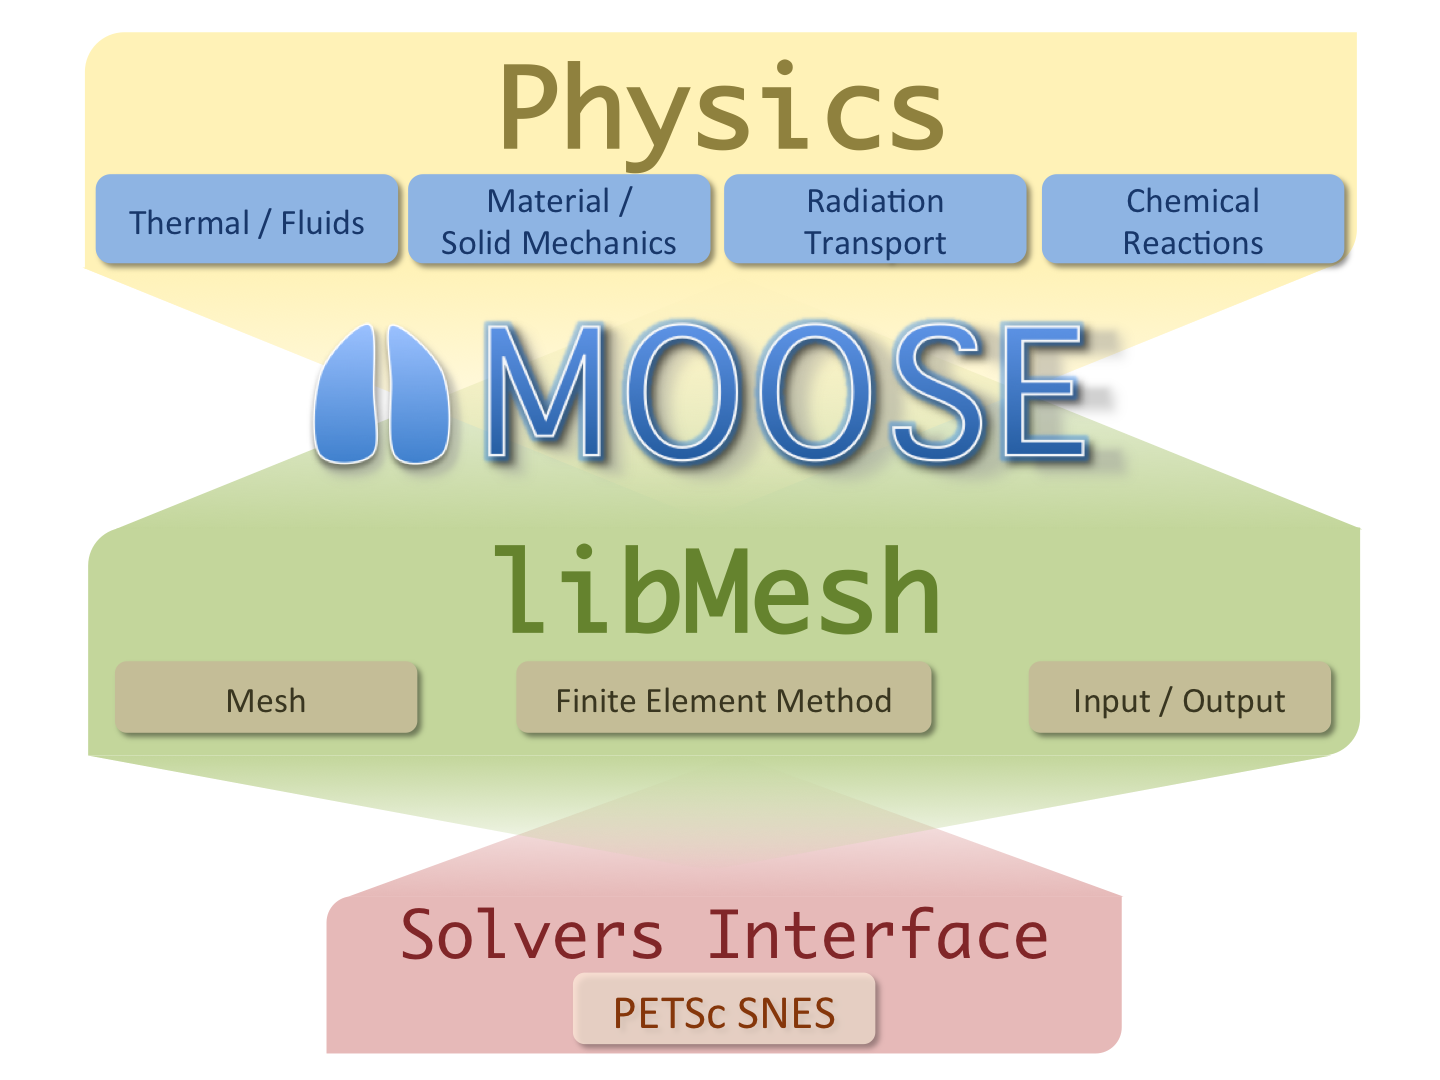
\includegraphics[height=0.8\textheight]{./images/moose_design.png}
          \caption{Shamelessly copied from the 
          \href{https://mooseframework.inl.gov/workshop/\#/2/4}{MOOSE Team Workshop slides}.}
    \end{figure}
\end{frame}


\begin{frame}
        \frametitle{How Does it Work?}
  \begin{figure}
   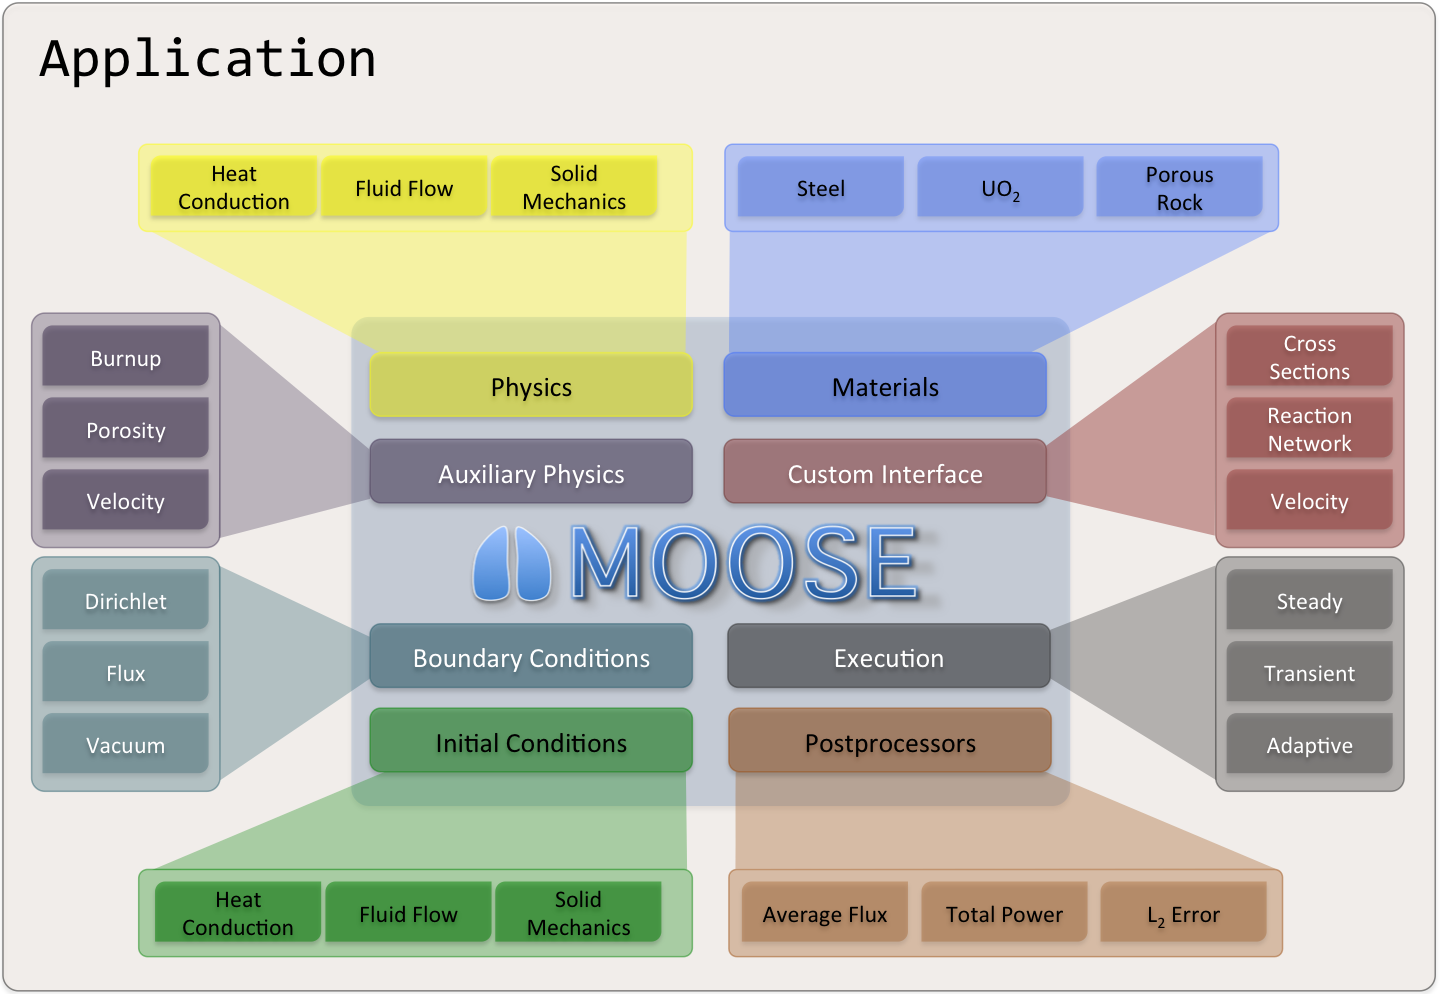
\includegraphics[width=0.9\textwidth]{./images/moose_systems.png}
          \caption{Shamelessly copied from the 
          \href{https://mooseframework.inl.gov/workshop/\#/2/6}{MOOSE Team Workshop slides}.}
    \end{figure}
\end{frame}

\begin{frame}
        \frametitle{How Does it Work?}
  \begin{figure}
   \vspace{-0.05in}
   \hspace*{-0.15in}
   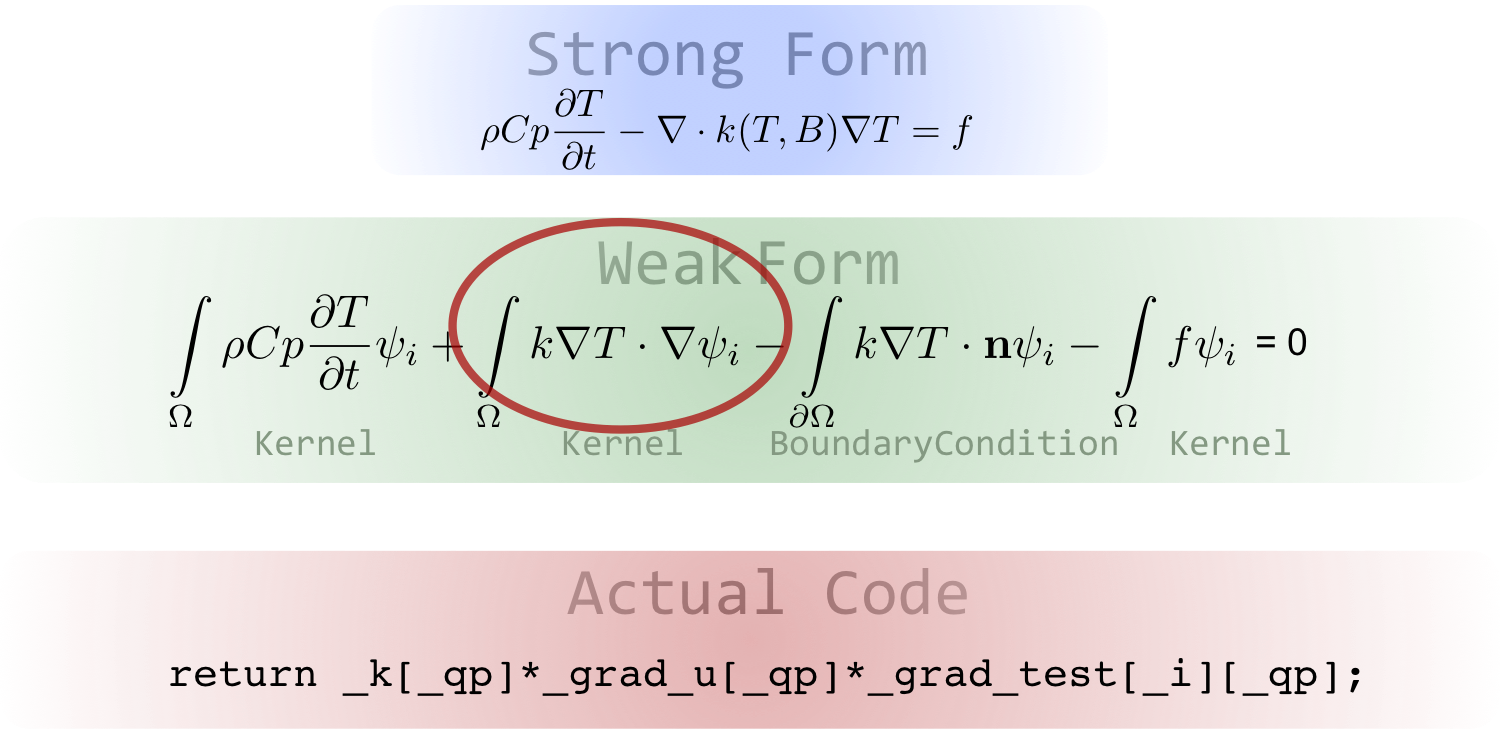
\includegraphics[width=\textwidth]{./images/moose_code.png}
          \caption{Shamelessly copied from the 
          \href{https://mooseframework.inl.gov/workshop/\#/2/7}{MOOSE Team Workshop slides}.}
    \end{figure}
\end{frame}

\begin{frame}
        \frametitle{MOOSE: Key Features}
        \begin{columns}
                \column[t]{5.5cm}
               \begin{itemize}
               \item MOOSE Framework is truly open source (LGPL)
               \item Developed initially for nuclear applications 
               \item Signficant long-term support from US DOE
               \item Continuous integration support (CIVET)
               \item Intuitive parallel multiscale solves
               \item Easy developer onboarding
               \end{itemize}
                \column[t]{5.5cm}
               \begin{itemize}
               \item Object Oriented, C++
               \item Interfaces with libMesh to discretize simulation volume into finite elements
               \item Residuals and Jacobians handed off to PetSc which handles solution of resulting non-linear system of algebraic equations
               \item Fully-coupled, fully-implicit multiphysics solver
               \item Automatically parallel (largest runs \textgreater 100,000 CPU cores!)
               \item Built-in adaptive meshing \& timestepping 
               \end{itemize}
        \end{columns}

\end{frame}

\begin{frame}
        \frametitle{Pros and Cons}
        \begin{columns}
                \column[t]{5.5cm}
                \textbf{Pros (+)}
               \begin{itemize}
               \item LGPL means the Framework is open, but apps can be restricted
               \item Vast array of available apps and kernels
               \item Many solver and preconditioning options
               \item Finite Element Modeling
               \item Full coupling is optional
               \item Generates gorgeous visualizations
               \end{itemize}
                \column[t]{5.5cm}
                \textbf{Cons (-)}
               \begin{itemize}
               \item LGPL means the Framework is open, but apps can be restricted
               \item Vast array of available apps and kernels
               \item Many solver and preconditioning options
               \item Finite Element Modeling
               \item Full coupling is optional
               \item Generates gorgeous visualizations
               \end{itemize}
        \end{columns}

\end{frame}

\section{Moltres (a MOOSE Application)}

\begin{frame}
        \frametitle{Moltres: Coupling in MOOSE}
  \begin{figure}
   \vspace{-0.05in}
   \hspace*{-0.15in}
   \includegraphics[width=1.1\textwidth]{./images/moltres-moose-diag.png}
    \end{figure}
\end{frame}


\begin{frame}
        \frametitle{Moltres: Basics}
        \begin{itemize}  
                \item Developed in ARFC group
                \item Fluid-fuelled, molten salt reactors
                \item Multi-group diffusion (arbitrary groups)
                \item Advective movement of delayed neutron precursors
                \item Navier-Stokes thermal hydraulics
                \item 3D unstructured
                \item 2D axisymmetric
                \item 3D structured 
                \item Initial developer: Alexander Lindsay \cite{lindsay_introduction_2018}
        \end{itemize}
\end{frame}

\begin{frame}
        \frametitle{Acquiring Moltres}
             \texttt{git clone https://github.com/arfc/moltres}\\
        \texttt{cd moltres}\\
        \texttt{git submodule init}\\
        \texttt{git submodule update}\\
\end{frame}

\begin{frame}
        \frametitle{Diffusion in Moltres}
        \footnotesize{
        \begin{align}
        \frac{1}{v_g}\frac{\partial \phi_g}{\partial t} &- \nabla \cdot D_g
        \nabla \phi_g + \Sigma_g^r \phi_g =\\
                &\sum_{g \ne g'}^G \Sigma_{g'\rightarrow g}^s \phi_{g'} + \chi_g^p \sum_{g' = 1}^G (1 -
        \beta) \nu \Sigma_{g'}^f \phi_{g'} + \chi_g^d \sum_i^I \lambda_i C_i
        \end{align}}
\begin{columns}
    \begin{column}{0.48\textwidth}
        \footnotesize{
        \begin{align*}
                v_g &= \mbox{speed of neutrons in group g} \\
                \phi_g &= \mbox{flux of neutrons in group g} \\
                t &= \mbox{time} \\
                D_g &= \mbox{Diffusion coefficient for neutrons in group g} \\
                \Sigma_g^r &= \mbox{macroscopic cross-section for}\\
                &\mbox{removal of neutrons from group g} \\
                \Sigma_{g'\rightarrow g}^s &= \mbox{macroscopic cross-section 
                of}\\
                &\mbox{  scattering from g' to g} \\
                \chi_g^p &= \mbox{prompt fission spectrum, neutrons in group g} \\
        \end{align*}}
    \end{column}
    \begin{column}{0.48\textwidth}
        %Content
        \footnotesize{
        \begin{align*}
                G &= \mbox{number of discrete groups, g} \\
                \nu &= \mbox{neutrons produced per fission} \\
                \Sigma_g^f &= \mbox{macroscopic fission cross section}\\
                &\mbox{ due to neutrons in group g} \\
                \chi_g^d &= \mbox{delayed neutrons in group g} \\
                I &= \mbox{ delayed neutron precursor groups} \\
                \beta &= \mbox{delayed neutron fraction}\\
                \lambda_i &= \mbox{average decay constant}\\
                &\mbox{of delayed neutron precursors in group i} \\
                C_i &= \mbox{concentration of delayed neutron}\\
                &\mbox{precursors in precursor group i}\\.
        \end{align*}}
    \end{column}
\end{columns}
\end{frame}

\begin{frame}
        \frametitle{Moltres Delayed Neutrons}
        \begin{align}
        \frac{\partial C_i}{\partial t} &= \sum_{g'= 1}^G \beta_i \nu
        \Sigma_{g'}^f \phi_{g'} - \lambda_i C_i - \frac{\partial}{\partial z} u
        C_i \label{eq:precursors}
\end{align}

        \begin{align*}
                G &= \mbox{number of discrete groups, g} \\
                I &= \mbox{ delayed neutron precursor groups} \\
                C_i &= \mbox{concentration of delayed neutron}\\
                &\mbox{precursors in precursor group i}\\.
                u &= \mbox{vertical fluid velocity}\\
                \lambda_i &= \mbox{average decay constant}\\
                &\mbox{of delayed neutron precursors in group i} \\
                \beta &= \mbox{fraction of delayed neutron}\\
                &\mbox{precursors in group i} \\
        \end{align*}
\end{frame}


\begin{frame}
        \frametitle{Moltres Fuel Temperature}
\begin{align}
        \rho_fc_{p,f}\frac{\partial T_f}{\partial t} &+ \nabla\cdot\left(\rho_f
        c_{p,f} \vec{u}\cdot T_f -k_f\nabla T_f\right) =  Q_f
\end{align}
\begin{align}
  \rho_f &= \mbox{density of fuel salt}\\
  c_{p,f} &= \mbox{specific heat capacity of fuel salt}\\
  T_f &= \mbox{temperature of fuel salt}\\
  \vec{u} &= \mbox{velocity of fuel salt}\\
  k_f &= \mbox{thermal conductivity of fuel salt}\\
  Q_f &= \mbox{source term} = \sum_{g=1}^G \epsilon_{f,g}\Sigma_{f,g}\phi_g
\end{align}
\end{frame}


\begin{frame}
        \frametitle{Moltres Moderator Temperature}
\begin{align}
        \rho_gc_{p,g}\frac{\partial T_g}{\partial t} &+
        \nabla\cdot\left(-k_g\nabla T_g\right) =  Q_g\\
\end{align}
\begin{align}
  \rho_g &= \mbox{density of graphite moderator}\\
  c_{p,g} &= \mbox{specific heat capacity of graphite moderator}\\
  T_g &= \mbox{temperature of graphite moderator}\\
  k_g &= \mbox{thermal conductivity of graphite moderator}\\
  Q_g &= \mbox{source term in graphite moderator}\\
\end{align}

\end{frame}


\begin{frame}
        \frametitle{Moltres MSRE Simulation}
  \begin{figure}
   \vspace{-0.05in}
   \includegraphics[height=0.85\textheight]{./images/msre.png}
    \end{figure}
\end{frame}


%\begin{frame}
%        \frametitle{Moltres MSRE Simulation}
%  \begin{figure}
%   \vspace{-0.05in}
%   \includegraphics[width=1.2\textwidth]{./images/moltres-input.png}
%          \caption{Data used in \cite{lindsay_introduction_2018}.}
%    \end{figure}
%\end{frame}

%\begin{frame}
%        \frametitle{Moltres MSRE Simulation}
%  \begin{figure}
%   \vspace{-0.05in}
%   \includegraphics[width=0.85\textwidth]{./images/moltres-composition.png}
%          \caption{Data used in \cite{lindsay_introduction_2018}.}
%    \end{figure}
%\end{frame}


\begin{frame}
        \frametitle{Mesh Generation for MOOSE Apps like Moltres}
  \begin{figure}
   \vspace{-0.05in}
   \includegraphics[height=0.85\textheight]{./images/lindsay_msre_moose.png}
    \end{figure}
\end{frame}



\begin{frame}
        \frametitle{Moltres Precursor Drift}
  \begin{figure}
   \vspace{-0.1in}
   \includegraphics[width=0.28\textwidth]{./images/auto_diff_rho_pre1.eps}
   \includegraphics[width=0.28\textwidth]{./images/auto_diff_rho_pre2.eps}
   \includegraphics[width=0.28\textwidth]{./images/auto_diff_rho_pre3.eps}
   \includegraphics[width=0.28\textwidth]{./images/auto_diff_rho_pre4.eps}
   \includegraphics[width=0.28\textwidth]{./images/auto_diff_rho_pre5.eps}
   \includegraphics[width=0.28\textwidth]{./images/auto_diff_rho_pre6.eps}
    \end{figure}
\end{frame}




\begin{frame}
        \frametitle{Moltres: More Complex Mesh}
  \begin{figure}[t]
   \vspace{-0.1in}
   \hspace*{-0.45in}
   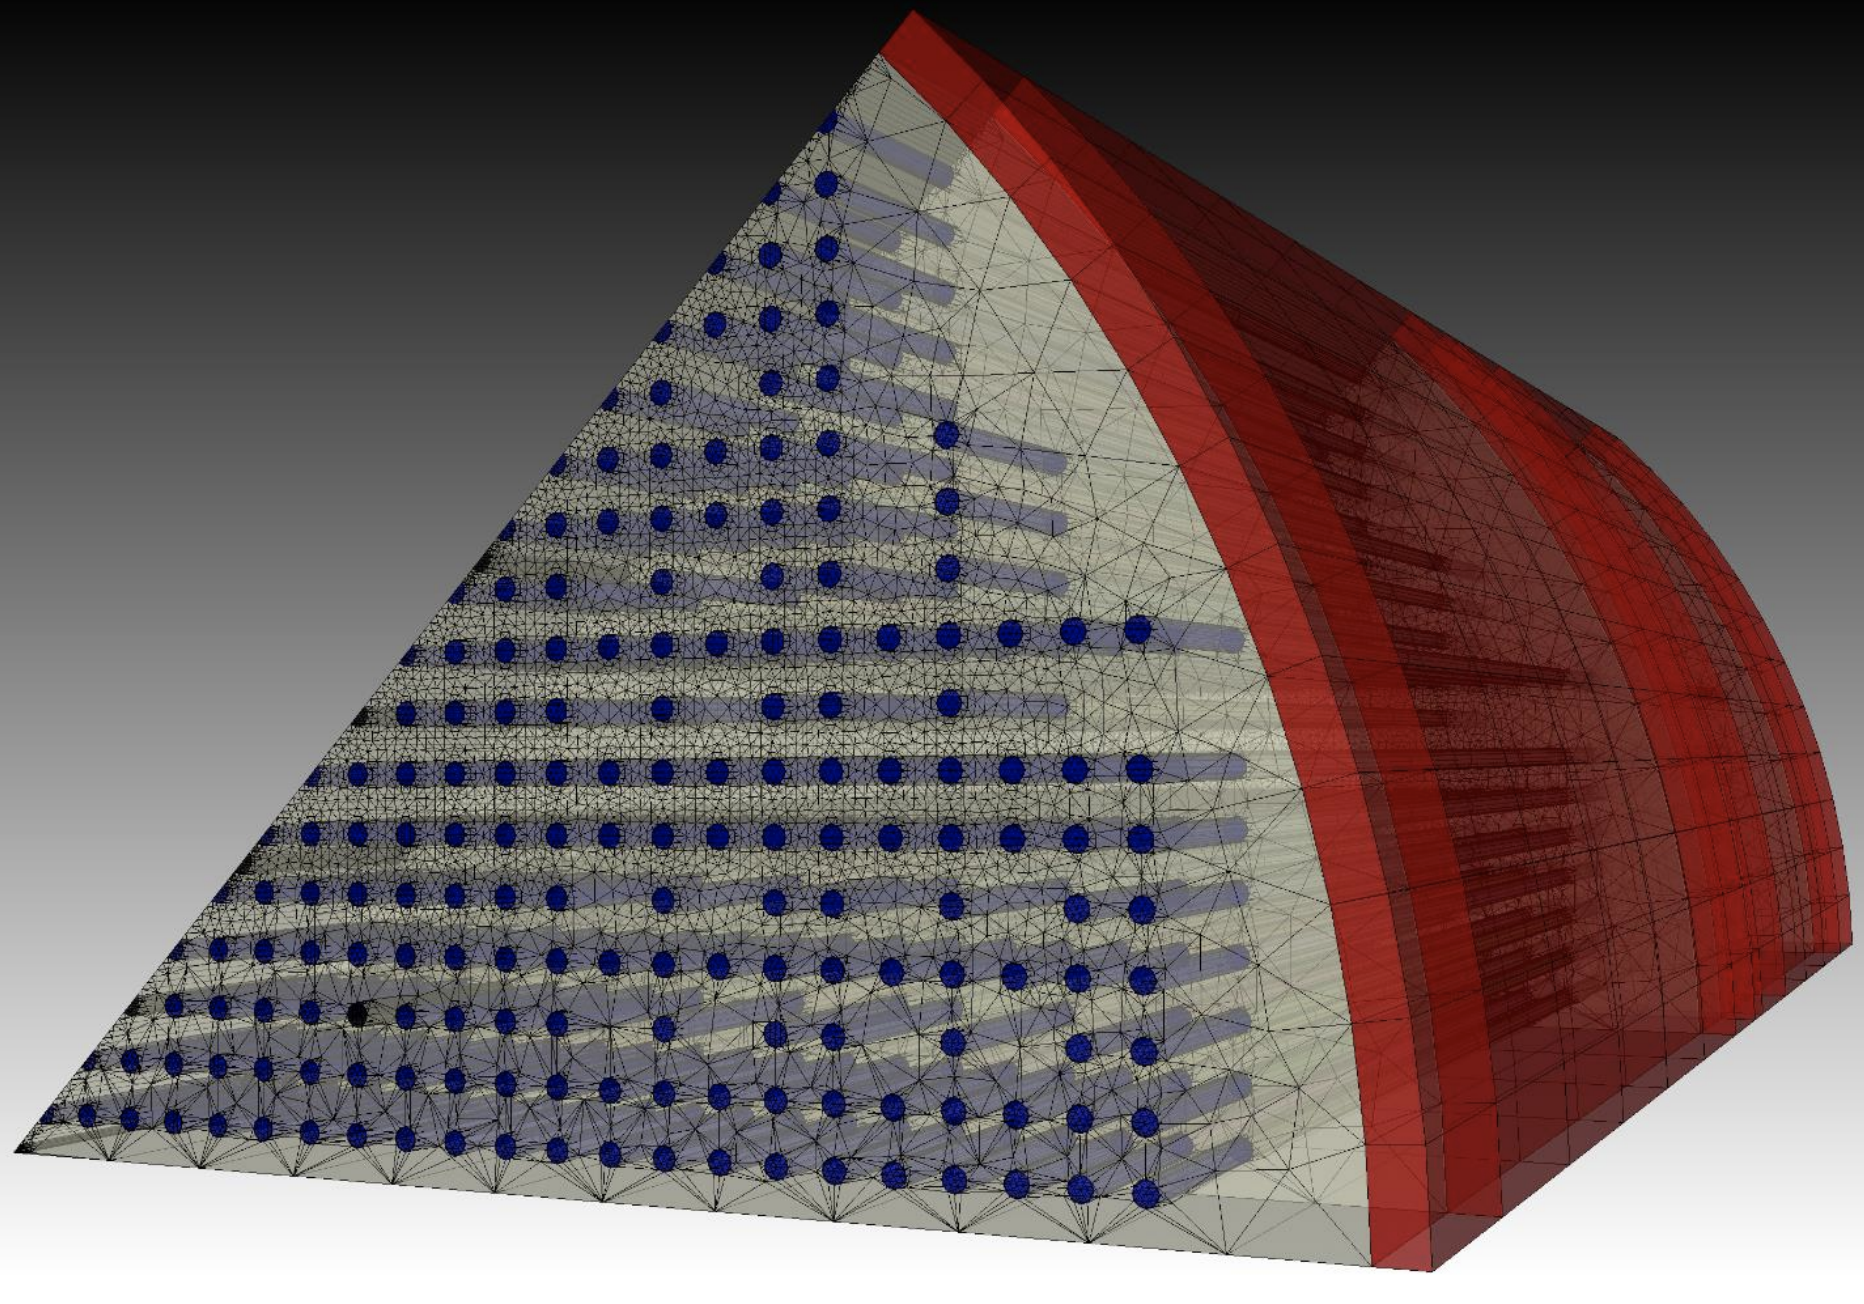
\includegraphics[height=0.75\textheight]{./images/lee-tap-mesh.png}
          \caption{TAP Mesh generated by Alvin Lee \cite{lee_neutronics_2020}. Red = Reactor Vessel Wall, Light Yellow =
Fuel Salt, Dark Gray = Control Rods, Blue = Fuel Salt radially co-located with 
          the Moderator Rods.}
    \end{figure}

\end{frame}

\begin{frame}
  \frametitle{Moltres: Multiphysics simulation (3D)}
  \begin{figure}[t]
   \vspace{-0.1in}
   \hspace*{-0.45in}
   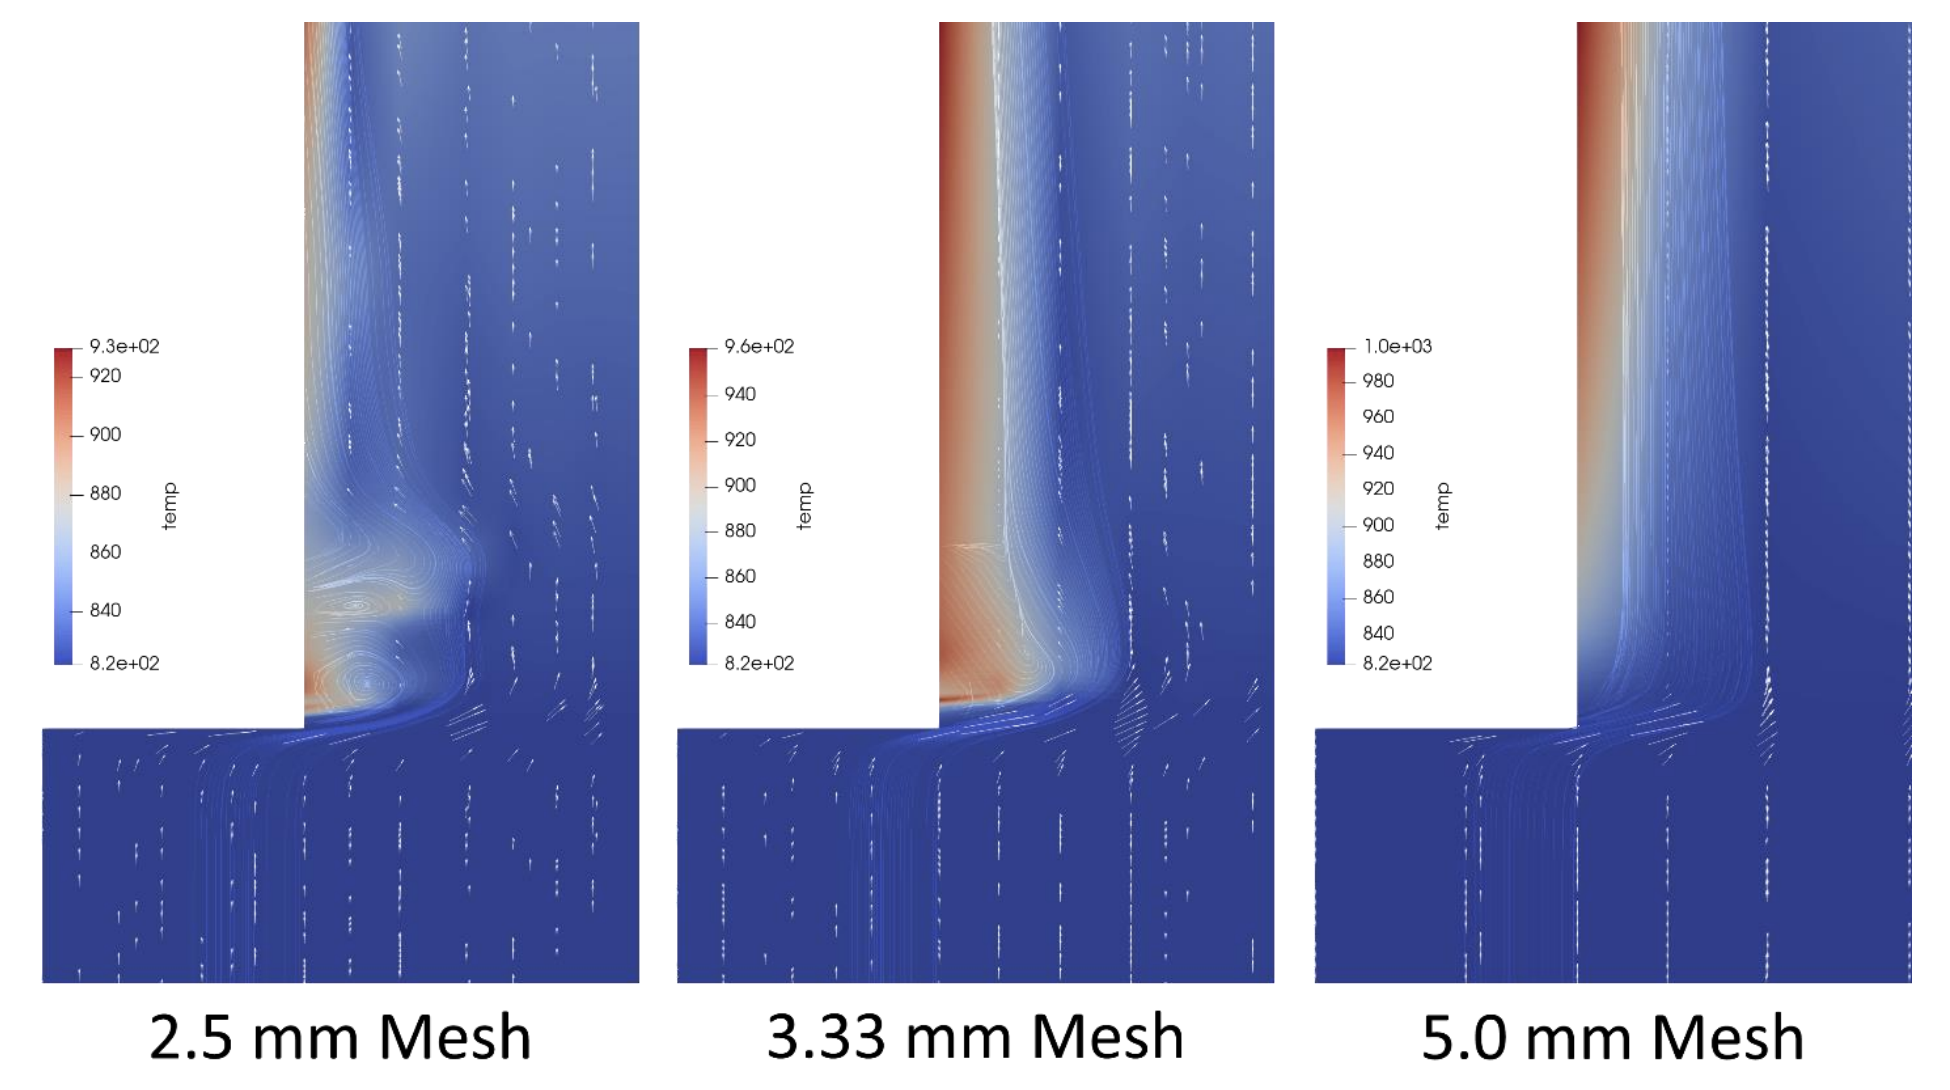
\includegraphics[height=0.75\textheight]{./images/lee-instability-resolution.png}
          \caption{Meshing study by Alvin Lee \cite{lee_neutronics_2020} 
          regarding KH instabilities and resolution of MSR fuel salt vortices.}
    \end{figure}

\end{frame}

\begin{frame}
        \frametitle{What now?}
        \textbf{Get Started}\\
        \href{https://mooseframework.inl.gov/}{https://mooseframework.inl.gov/}
        \href{https://github.com/idaholab/moose}{https://github.com/idaholab/moose}\\
        \href{https://github.com/arfc/moltres}{https://github.com/arfc/moltres}\\
        \textbf{Other Tools}\\
        \href{https://gmsh.info/}{https://gmsh.info}\\
        \href{https://github.com/pyne/pyne}{https://github.com/pyne/pyne}\\
        \href{https://github.com/openmc-dev/openmc}{https://github.com/openmc-dev/openmc}\\
        \href{https://www.paraview.org}{https://www.paraview.org}

\end{frame}

\input{moltres}
\begin{frame}
  \frametitle{Conclusion}
        We showed many things. This slide is an example of how 
        you can animate bulletted lists, for more information about
        using beamer animations, checkout the overleaf article on 
        overlay specifications in the group's guide.
        \begin{itemize}
                \item Cats are peculiar
                \pause
                \item Blue and Orange are fierce colors
                \pause
                \item Math can be rendered nicely
                \pause
                \item Cite your sources
        \end{itemize}
\end{frame}

\begin{frame}
  \frametitle{Acknowledgements}
  \begin{itemize}
    \item This research is part of the Blue Waters sustained-petascale computing project, 
which is supported by the National Science Foundation (awards OCI-0725070 and 
ACI-1238993) and the state of Illinois.
    \item Kathryn Huff is additionally supported by the NRC Faculty Development Program, the NNSA (awards 
    DE-NA0002576 and DE-NA0002534), and the International Institute for Carbon Neutral Energy Research (WPI-I2CNER).
    \item The authors would like to thank  members of Advanced Reactors and Fuel Cycles
research group (ARFC) at the University of Illinois at Urbana Champaign who 
provided valuable code reviews and proofreading.
    \item This work is derived from the work of Alex Lindsay (Idaho National Laboratory), Gavin Ridley (University of 
            Tennessee-Knoxville), Andrei Rykhlevskii (Argonne National 
                  Laboratory), Sun Myung Park (UIUC), and Alvin Lee (UIUC).
  \end{itemize}
    \begin{figure}[t]
   \hspace*{-0.4in}
   \includegraphics[height=0.25\textheight]{./images/acks.png}
    \end{figure}
\end{frame}

%%--------------------------------%%
%%--------------------------------%%
\begin{frame}[allowframebreaks]
  \frametitle{References}
  \bibliographystyle{plain}
  {\footnotesize \bibliography{2021-huff-iaea} }

\end{frame}


%%---BACKUP SLIDES----------------%%

\begin{frame}
\frametitle{Online reprocessing method}
  \begin{columns}
    \column[t]{6cm}
	\begin{figure}[t]
                \vspace*{-0.35in}
			\hspace{-0.3in}
                 \includegraphics[height=\textwidth]{./images/saltproc_flowchart.pdf}
                \vspace*{-0.05in}
                \caption{Flow chart for the SaltProc.}
      \end{figure}

    \column[t]{6cm}
             \begin{block}{SaltProc capabilities}
               \begin{itemize}             
               \item Remove specific isotopes from the core with specific parameters (reprocessing interval, mass rate, removal efficiency)
               \item Add specific isotopes into the core
               \item Maintain constant number density of specific isotope in the core
	       \item Store stream vectors in an HDF5 database for further analysis or plots
	       \item Generic geometry: an infinite medium, a unit cell, a multi-zone simplified assembly, or a full-core
               \end{itemize}
               \end{block}
  \end{columns}
\end{frame}

\begin{frame}
  \frametitle{Online reprocessing method}
     \begin{figure}[t]
                \vspace*{-0.1in}
                  % \hspace*{-0.37in}
                \includegraphics[height=0.45\textwidth]{./images/pa_isolation.png}
                \vspace*{-0.09in}
                \caption{Protactinium isolation with uranium removal by fluorination \cite{robertson_conceptual_1971}.}
      \end{figure}
                      \vspace*{-0.22in}
             \begin{block}{Online reprocessing approach}
               \begin{itemize}             
               \item Continuously removes all poisons, noble metals, and gases.
               \item $^{233}$Pa is continuously removed from the fuel salt into a decay tank.
               \end{itemize}
               \end{block}
               \vspace{-0.05in}
$\qquad\qquad\qquad\qquad^{232}_{90}$Th+$^1_0$n$\rightarrow^{233}_{90}$Th$\xrightarrow[\text{22.3 min}]{\beta^-}$ $^{233}_{91}$Pa$\xrightarrow[\text{26.967 d}]{\beta^-}$ $^{233}_{92}$U
\end{frame}


%        File: arfc-pres.tex
\begin{frame}
  \frametitle{Effective multiplication factor for full-core \gls{MSBR} model }
    \begin{columns}
    \column[t]{7cm}
   \vspace{-0.35in}
  \begin{figure}[t]
   \hspace*{-0.2in}
   \includegraphics[height=0.75\textheight]{./images/keff.png}
   \vspace{-0.05in}
   \caption{$k_{eff}$ during a 20 years depletion simulation.}
    \end{figure}

    \column[t]{4.5cm}
       \begin{itemize}
	        \item Strong absorbers ($^{233}$Th,$^{234}$U) accumulating in the core
   		\item Fissile materials other than $^{233}$U are bred into the core ($^{235}$U, $^{239}$Pu)
   		\item The multiplication factor stabilizes after approximately 6 years
       \end{itemize}
     \end{columns}
\end{frame}

\begin{frame}
  \frametitle{Power and breeding distribution}
    \begin{columns}
    \column[t]{6cm}
  \begin{figure}[t]
   \vspace{-0.25in}
   \hspace*{-0.15in}
   \includegraphics[height=0.6\textheight]{./images/power_distribution.png}
   \vspace{-0.1in}
   \caption{Normalized power density}
    \end{figure}

    \column[t]{6cm}
  \begin{figure}[t]
   \vspace{-0.25in}
	\hspace*{-0.05in}
   \includegraphics[height=0.6\textheight]{./images/breeding_distribution.png}
   \vspace{-0.1in}
   \caption{$^{232}$Th neutron capture reaction rate normalized by total flux}
    \end{figure}

     \end{columns}
\end{frame}

\begin{frame}
  \frametitle{$^{232}$Th refill rate}
    \begin{columns}
    \column[t]{7cm}
   \vspace{-0.35in}
  \begin{figure}[t]
   \hspace*{-0.2in}
   \includegraphics[height=0.75\textheight]{./images/Th_refill_rate.png}
   \vspace{-0.05in}
   \caption{$^{232}$Th feed rate over 20 years of \gls{MSBR} operation}
    \end{figure}

    \column[t]{4.5cm}
       \begin{itemize}
	        \item Fluctuation due to batch-wise removal of strong absorbers
   		\item Feed rate varies due to neutron energy spectrum evolution
   		\item $^{232}$Th consumption is 100 g/GWh$_e$
       \end{itemize}
     \end{columns}
\end{frame}



\begin{frame}
  \frametitle{Multiplication factor dynamics during Rb, Sr, Cs, Ba removal (3435days)}
               \begin{figure}[t]
                \vspace*{-0.1in}
                \includegraphics[height=0.7\textwidth]{./images/keff_3435st.png}
               \end{figure}

\end{frame}


\begin{frame}
  \frametitle{\gls{MSBR} neutron energy spectrum for different regions}
               \begin{figure}[t]
                \vspace*{-0.1in}
                \includegraphics[height=0.35\textwidth]{./images/spectrum_zones_init.png}
               \end{figure}
               \begin{figure}[t]
                \vspace*{-0.1in}
                \includegraphics[height=0.35\textwidth]{./images/spectrum_zones_eq.png}
               \end{figure}

\end{frame}

\begin{frame}
  \frametitle{Fissile isotopes in the \gls{MSBR} core}
  \begin{columns}
    \column[t]{6cm}
               \begin{figure}[t]
                \vspace*{-0.1in}
                \includegraphics[height=0.75\textwidth]{./images/fissile_short.png}
               \end{figure}
    \column[t]{6cm}
               \begin{figure}[t]
                \vspace*{-0.1in}
                \includegraphics[height=0.75\textwidth]{./images/fissile_long.png}
               \end{figure}
    \end{columns}
\end{frame}
\end{document}
